\documentclass[runningheads]{llncs}

%---- Sonderzeichen-------%
\usepackage[ngerman]{babel}
%---- Codierung----%
\usepackage[utf8]{inputenc}
%\usepackage[latin1]{inputenc}
\usepackage[T1]{fontenc}
\usepackage{graphicx}
\usepackage{url}
\usepackage{llncsdoc}
%----- Mathematischer Zeichenvorrat---%
\usepackage{amsmath}
\usepackage{amssymb}
\usepackage{enumerate}
% fuer die aktuelle Zeit
\usepackage{scrtime}
\usepackage{listings}
\usepackage{subfigure}
\usepackage{hyperref}
\usepackage{lipsum}

\setcounter{tocdepth}{3}
\setcounter{secnumdepth}{3}

% -- CUSTOM ADDITIONS --

%% Use glossaries (optional)
\makeglossaries
% %% Load glossary definitions from file
\loadglsentries{glossentries.tex}

% Proper Table line breaks
\usepackage{tabularx}
% Syntax highlighting
\usepackage{listings}

% -- END CUSTOM ADDITIONS --

% -------------------------------------------------------------------------------------------------
% -------------------------------------------------------------------------------------------------
\begin{document}

\mainmatter
\title{Cloud und Edge Robotics}
\titlerunning{Cloud und Edge Robotics}
\author{Daniel Vera Gilliard}
\authorrunning{Vertiefungsseminar Internet of Things}
\institute{Betreuer: Prof. Dr. rer. nat. Christian Zirpins}
\date{22.11.2022}
\maketitle

% -------------------------------------------------------------------------------------------------

\begin{abstract}
  Das Thema Cloud und Edge Robotics umfasst Themenbereiche rund um die Robotik Systeme, dem Edge Layer und der Cloud. Daraus ergeben sich interessante Use Cases und Herausforderungen die in dieser Arbeit untersucht werden. Das Ziel in der vorliegenden Seminararbeit ist es, eine Auswahl an Konzepten und Technologien im Edge und Cloud Robotics Bereich vorzustellen und zu bewerten. Dazu wird auf deren Eigenschaften in Bezug auf den Robotics Bereich eingegangen und beispielhafte Use Cases vorgestellt. Als Grundlage, wurden dabei relevante Wissenschaftliche Arbeiten sowie aktuelle Technologien ausgewertet. Daraus stellten sich das \acrfull{ros2} mit dem \acrfull{dds}, so wie das Netzwerkprotokoll Zenoh als wichtige Werkzeuge um das Konzept des \acrlong{cttc} zu realisieren. Zenoh ermöglicht dabei eine performante und skalierbare Kommunikation zwischen Robotern dem Edge und der Cloud. Die vorgestellten Technologien ergeben ein großes Potential, um Robotik Projekte einfacher mit der Edge und Cloud zu integrieren. Durch die schnelllebige Entwicklung rund um die Cloud und das Edge Robotics Thema, empfiehlt es sich jedoch weitere sich noch in der Entwicklung befindliche Technologien mitzuverfolgen. 
\end{abstract}

% -------------------------------------------------------------------------------------------------

\section{Einleitung}
\label{sec:Einleitung}

Die Robotik und die Themenbereiche rund um die Cloud und das Edge Computing sind sehr relevant für die Zukunft.\\
Die Robotik bietet dabei eine große Bandbreite an Anwendungsmöglichkeiten. Diese erstrecken sich von regulären Haushaltsrobotern bis hin zum Einsatz in speziellen Industriellen Anwendungsgebieten. Dies zeigt sich eindrucksvoll an der erst im Oktober 2022 veröffentlichten Statistik der International Federation of Robotics in der die Nutzung von Robotern im Professionellen Kontext um  37\% im Jahre 2021 gestiegen ist \cite{ifrSalesRobotsService2022} . Im Haushaltskontext gab es dabei eine Erhöhung von 12\% in den Verkaufszahlen.\\
Die Cloud und speziell der Bereich des Edge Computing spielen im Alltag und im Kommerziellen Umfeld ebenfalls eine entscheidende Rolle. Die Cloud bietet dabei die Möglichkeit auf unterschiedliche Computer Ressourcen über das Internet zuzugreifen und diese bei Bedarf einfach zu skalieren \cite{mellNISTDefinitionCloud} . Das Edge Computing fokussiert sich dabei auf die Anwendungsfälle am Rande des Netzwerks und ist ein wichtiger Bestandteil in der Umsetzung von Themenbereichen wie das Autonome Fahren oder Smart Cities.

Neben denen im letzten Absatz angesprochenen Themenbereiche, profitiert auch die Robotik von der Entwicklung im Bereich des Cloud und Edge Computing. Im speziellen, kann es hier die Ressourcen in der Cloud oder Edge nutzen, um die Funktionalität zu verbessern oder die gesammelten Daten besser zu nutzen.\\
Die in dieser Arbeit thematisierten Aspekte, orientieren sich an dem von Milan Groshev et al. (2015) \cite{groshevEdgeRoboticsAre2022} evaluierten Zustandes im Cloud und Edge Robotics Bereich. Im Folgenden, wird die Motivation hinter der Kombination beider Technologien erläutert, die Herausforderungen definiert und eine Übersicht über die untersuchten Lösungsansätze präsentiert die man in der Praxis nutzen kann.

\subsection{Struktur der Arbeit} % (fold)
\label{sub:Struktur der Arbeit}

Diese Arbeit ist in drei Teilen aufgebaut. Im ersten Teil wird eine Hinführung auf die für diese Arbeit nötigen Grundlagen gegeben. Dazu werden Konzepte aus den Bereichen der Cloud und dem Edge eingeführt. Es werden ebenfalls die Eigenschaften von Robotik Systemen beschrieben und mit dem \acrlong{ros} das aktuell gängige System zur Nutzung in der Robotik vorgestellt. Um die Schnittstelle zum Cloud und Edge Bereich herzustellen, wird hier ein Fokus auf die verwendeten Kommunikationsprotokolle in der Robotik gesetzt.\\
Der Hauptteil Gliedert sich in vier Abschnitte. Zu Beginn wird erklärt, wie die Zusammenführung von der Cloud, dem Edge und Robotern funktionieren kann und welche Vorteile man aus dem Zusammenschluss bekommen kann. Im folgenden, wird ein Blick auf die Einbindung der Roboter in das Gesamtsystem durch das Zenoh Protokoll gesetzt. Nach den eher spezielleren Themen, wird in den letzten beiden Abschnitten vom Hauptteil eine übergeordnete Sicht auf das Thema Cloud und Edge Robotics gemacht. Dazu werden allgemeine Architekturen betrachtet. Darauf aufbauend, werden verschiedene Use Cases vorgestelt die eine praktische Anwendung zeigen sollen.\\
Die Arbeit wird mit dem Fazit abgeschlossen. Hier wird ein Ausblick auf Technologien und die Weiterentwicklung in der Forschung und Entwicklung von Bereichen im Cloud und Edge Robotics Spektrum gemacht. Schließlich wird das ganze durch ein Fazit über die behandelten Themen beendet.

% subsection Struktur der Arbeit (end)



\subsection{Motivation}

Wie man der Einleitung entnehmen konnte, steigt die Nutzung von Robotern kontinuierlich. Vor allem in der Industrie stellt sich dabei die Frage, wie man eine große Anzahl an Robotern in Produktion skalieren, in instabilen Umgebungen produktiv betreiben oder mit etablierten Cloud Lösungen integrieren kann. Beim Versuch diese Fragen zu beantworten, stößt man zwangsläufig auf Herausforderungen die im Zusammenhang mit der Nutzung von Robotern untereinander oder in Verbindung mit externen Services stehen.\\
Bei den genannten Herausforderungen geht es um verschiedene Bereiche. Zum einen natürlich um die zusammenarbeit Heterogener Systeme untereinander. Diese müssen fähig sein, miteinander interagieren zu können und zu kommunizieren. Wenn man noch die Cloud und Edge Server miteinbezieht, kommen noch weitere Systeme dazu die man berücksichtigen muss. Zum anderen, kommen hier auch die Cloud und Edge Systeme durch ihre unterschiedlichen Eigenschaften zur Geltung. Im Cloud Bereich, hat man dabei homogene Ressourcen die kurze Zyklen durchlaufen. Außerdem hat man eine hohe Verfügbarkeit. Im Edge Bereich ist genau das Gegenteil der Fall. Ressourcen sind sehr Heterogen, haben lange Lebenszyklen und die Verfügbarkeit ist sehr Variabel.\\
Neben der Art der Ressourcen, sind auch die Eigenschaften des Netzwerkes eine konstante Herausforderung. Ziel ist es dabei einen hohen Durchsatz sowie eine niedrige Latenz zu haben. Dies ist aber aufgrund der Art des Netzwerkes oft nicht möglich. Vor allem im Bereich der Robotik, muss man mit Drahtlosen, unzuverlässige Verbindungen umgehen.\\
Zu den Netzwerkherausforderungen kommen schließlich noch die Herausforderungen die sich durch die Topologie ergeben. Diese ergeben sich durch die große Anzahl an Beweglichen Knoten die im System vorhanden sind und die Geographische Verteilung die diese haben können.\\
Die Fragestellung dieser Arbeit setzt sich also aus den hier geschilderten Fragen zusammen. Dabei ist zu klären wie man mit den verschiedenen Herausforderungen umgehen kann und mit welcher Lösung man die verschiedenen Komponenten am besten in Einklang bringt.\\



% -------------------------------------------------------------------------------------------------

\section{Grundlagen}
\label{sec:grundlagen}

In dieser Seminararbeit werden verschiedene Technologien verwendet die für die Anwendung im Cloud und Edge Robotics Bereich relevant sind. Darunter befinden sich breitere Themenbereiche wie die Cloud oder das Edge Computing. Es werden aber auch speziellere Technologien wie ROS2 oder Zenoh für die Nutzung mit Robotern oder zur Kommunikation betrachtet. In diesem Abschnitt werden die Grundbegriffe und Technologien rund um das Cloud und Edge Robotics vorgestellt und im Kontext erläutert.

\subsection{Cloud-To-Thing Kontinuum} % (fold)
\label{sub:Cloud-To-Thing-Continuum}

Das \acrlong{cttc} beschreibt die Möglichkeit zur Nutzung von Speicher und Rechenkapazitäten, sowie der Sammlung von Daten auf einem Kontinuum. Das Kontinuum enthält, wie in \cite{cominardiDevopsEdgeopsVision2021} beschrieben, verschiedene Arten von Ressourcen die sich in mehreren Netzwerken oder geographischen Orten befinden. Die Ressourcen reichen von Roboter, über Edge Server bis hin zu Cloud Instanzen.

\begin{figure}
  \begin{center}
    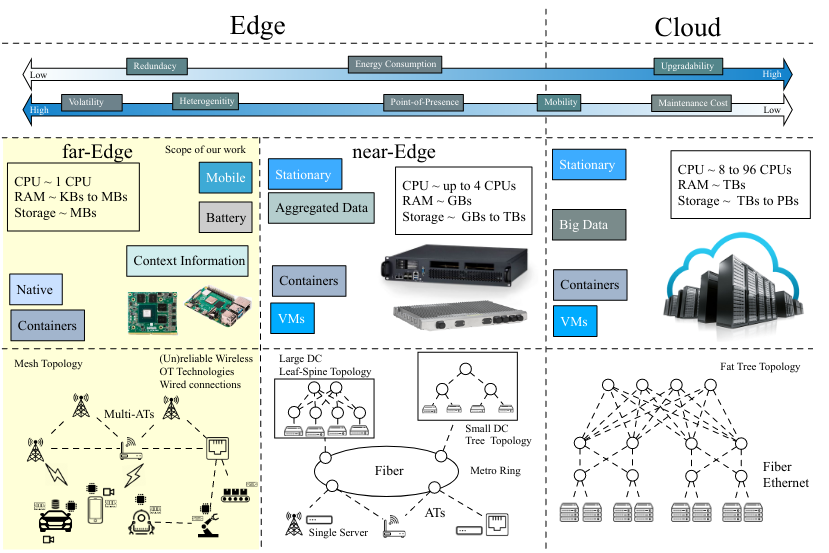
\includegraphics[width=0.95\textwidth]{./figures/cloud-thing-continuum.png}
  \end{center}
  \caption{Übersicht \acrlong{cttc} \cite{baldoniManagingFarEdgeAre2021}}
  \label{fig:cttc}
\end{figure}

Wie man in der Grafik \ref{fig:cttc} erkennen kann, hat man unterschiedliche heterogene Ressourcen die verschiedene Eigenschaften haben und unter verschiedenen Bedingungen agieren. Auf der einen Seite, hat man am Edge ein sehr heterogenes System mit Beispielsweise Robotern und IoT Geräten. Diese besitzen eingeschränkte Ressourcen wie Beispielsweise Rechenkapazitäten. Hinzu kommen unverlässliche Verbindungen wie Wi-Fi oder Bluetooth.\\
Auf der anderen Seite, befinden sich die Cloud Instanzen. Dessen Ressourcen sind recht homogen und verlässlich. Größtenteils also das genaue Gegenteil zu den Geräten nahe dem Edge. Zwischen den beiden Schichten befinden sich oftmals Edge Server. Diese ähneln den Komponenten der Cloud. Da sie aber von der Lokalität nahe an den Endgeräten sein müssen, sind Sie nicht so einfach Skalierbar wie Cloud Ressourcen.\\
Aufgrund der unterschiedlichen Gegebenheiten und Eigenschaften der Geräte, ist es wichtig ein einheitliches Kommunikationsmedium zu nutzen welches die Komponenten der verschiedenen Schichten unterstützt. Im Bereich der Robotik, wurden diese Aspekte ende 2018 in \cite{jawharNetworkingMultiRobotSystems2018} untersucht. Im Artikel wurde das \acrlong{cttc} als R2I(robot-to-infrastructure) beschrieben. Dabei wurden MRS(Multi-Robot-Systems) und die Möglichkeiten der Kommunikation verglichen. Beim Vergleich kamen die Autoren zu einer Ähnlichen Schlussfolgerung wie eingangs erwähnt: "This gateway node must be able to map the networking parameters associated with the data traffic in the data link layer header to the corresponding data link layer header in the infrastructure network." \cite{jawharNetworkingMultiRobotSystems2018}. Gemeint, sind die verschiedenen Protokolle die unterstützt werden müssen um sowohl Robotik als auch weitere Infrastruktur Systeme miteinander zu verbinden. Das Paper beschreibt zudem Grundprotokolle wie Wi-Fi oder Bluetooth die zum Austausch der Nachrichten benötigt werden. Wie man an den zahlreichen im Paper genannten Technologien erkennen kann, ist der Bereich um die Kommunikation im Robot to Infrastructure Bereich sehr Komplex. Das \acrlong{cttc} zielt dabei auf eine Vereinheitlichung der Kommunikationswege aus. Dabei wird eine Technologie gesucht, die bereits bestehende Protokolle unterstützt, abstrahiert oder ersetzt und als Ende zu Ende Lösung genutzt werden kann. Im folgenden Teil dieser Arbeit wird sich dieser Frage gewidmet.


\subsection{Edge Computing}

Das Ziel hinter Edge Computing ist es zum einen, Rechen oder Speicher Ressourcen näher an die Clients zu bringen. Edge Computing Server dienen dabei als Schnittstelle zwischen IoT Geräten und Datenzentren die sich in der Cloud befinden können \cite{luntovskyyHighlyDistributedSystemsIoT2022}.\\
Das Konzept wurde im modernen Kontext erstmals 2012 in einem Paper von dem Unternehmen Cisco vorgestellt \cite{bonomiFogComputingIts}. Dabei wurde es als Erweiterung der Cloud zur Unterstützung von Internet of Things (IoT) Anwendungen definiert. Anzumerken sei, dass im Paper der Begriff 'Fog' für 'Edge' genutzt wird. Beide werden in der Literatur oftmals als Synonym genutzt. In dieser Arbeit, wird der Begriff 'Edge' eingesetzt.\\
Wie also beschrieben, ist das Edge Computing eine besondere Art der Bereitstellung von Ressourcen für Clients. Aus diesem Grund, kann man mehrere Eigenschaften ausmachen die für das Edge computing von Bedeutung sind\cite{bonomiFogComputingIts}:

\begin{enumerate}
  \item Standorts Bewusstsein und geringe Latenz: Edge Knoten werden vornehmlich in der Näher von Clients plaziert. Dadurch können diese entlastet werden ohne dass es zu großen Latenz Problemen kommt.
    \item Geografische Verteilung: Um die nähe der Clients zu gewährleisten, werden die Edge Knoten an verschiedenen Orten angebracht. Dies muss beim Deployment der Knoten beachtet werden.
      \item Beweglichkeit: Im gegensatz zu stationäre Server, sind Edge Instanzen in Ihrem Ort beweglich. Dies ist nötig um Clients an unterschiedlichen Orten zu unterstützen und flexibel zu bleiben. Dafür wird ein System gebraucht welches den jeweiligen Edge Host von seinem Ort entkoppelt und Änderungen am Standort wahrnimmt und unterstützt.
        \item Echtzeit Kommunikation: Edge Knoten müssen in Echtzeit mit Endanwendungen kommunizieren können. Eine Verarbeitung in Form von zum Beispiel eine Warteschlange ist hier nicht möglich, da Clients auf die Antwort des Edge Servers womöglich angewiesen sind.
\end{enumerate}

Edge Computing unterscheidet sich dabei in verschiedenen Aspekten vom regulären Cloud Computing. Verbindungen haben in diesem Kontext oftmals eine viel größere Lebensspanne. Das heißt, dass die Verbindungen nicht wie bei regulären Internetdiensten nach einer kurzen Zeit wieder geschlossen werden. Ebenfalls, gibt es im Bereich des Edge Computings sehr viele heterogene Clients. Im Kontext der Robotik, könnte man zum Beispiel Verbindungen von einem mobilen Roboter und einem stationären Greifarm unterscheiden. Besonders eindrucksvoll ist dies im IoT Bereich, in dem man sehr viele verschiedene Verbindungen verarbeiten muss.\\
Diese Eigenschaften haben verschiedene Vorteile gegenüber dem regulären Cloud Computing. Einerseits, kann eine kürzere Distanz zum Server die Latenz der Verbindungen verbessern. Andererseits, kann es zu einer direkten Datenannahme und Pre-Prozessierung der Daten direkt am Standort kommen. Dies ist hilfreich, wenn die Datenverarbeitung für die Funktionalität des Roboters von Relevanz ist \cite{luntovskyyHighlyDistributedSystemsIoT2022}.

\begin{figure}
  \centering
  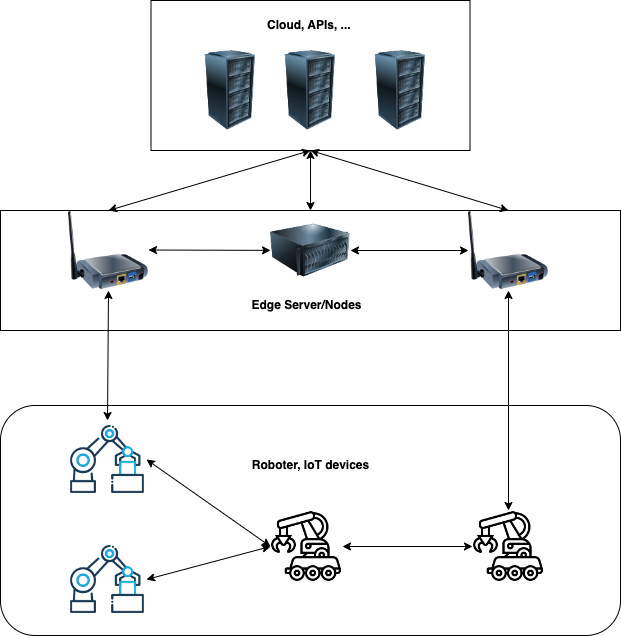
\includegraphics[width=0.5\textwidth]{./figures/edge-computing.png}
  \caption{Vereinfachte Edge Computing Architektur}
  \label{fig:edge-computing}
\end{figure}

Trotz der Allgegenwärtigkeit von Cloud Computing Services in unserem Alltag\cite{GartnerForecastsWorldwide2022}, gibt es im Edge Computing Bereich noch einige Herausforderungen. Eine davon ist die Konnektivität zwischen den Edge Knoten und den jeweiligen Geräten wie beispielsweise den Robotern. Das Wunschszenario wären hier hohe Datenraten mit möglichst niedrigen Verbindungsverzögerungen \cite{groshevEdgeRoboticsAre2022}. Dies ist aber oftmals durch äußere Einflüsse nicht reibungslos möglich. Beispielsweise spielt die Standort Wahrnehmung hier eine Rolle. Ein Roboter, der sich näher am Edge Knoten befindet kann auch von einer besseren Konnektivität profitieren.

Ziel ist es also die Zusammenarbeit zwischen Heterogene Ressourcen wie beispielsweise Roboter und Edge Knoten zu verbessern. Dafür müssen verschiedene Variablen berücksichtigt werden. Unter anderem die Konnektivität, die geographische Verteilung der Knoten oder der spezielle Use Case der umgesetzt werden soll.\\
In \ref{fig:edge-computing} ist eine vereinfachte Edge Architektur dargestellt. Hier hat man in der untersten Schicht mehrere Roboter die Dienste von einer Edge Instanz nutzen. Die Edge Instanzen können sich dabei direkt bei den Robotern befinden (Bspw. in einer Fabrik) oder nur geographisch an einem nähern Ort als Cloud Server. Durch die nähere Distanz ist aus performance Sicht eine Auslagerung überhaupt möglich. In der obersten Schicht, sind die für Roboter Betriebs irrelevante Services angesiedelt. Diese können zum Beispiel Cloud Schnittstellen sein, die Berechnungen anhand der gesammelten Daten an der Edge ausführen.


\subsection{Cloud Computing}

Cloud Computing ist ein sehr großer und weitreichender Begriff der in den letzten Jahren sehr stark gewachsen ist. Rimal et al. \cite{rimalArchitecturalRequirementsCloud2011} beschreibt Cloud Computing folgendermaßen: "Cloud Computing is a model of service delivery and access where dynamically scalable and virtualized resources are provided as a service over the Internet.". Wie in der Definition erwähnt, bietet Cloud computing einen großen Vorteil gegenüber traditionellen, selbst betriebene Servern. Bei Cloud Computing hat man dabei zum einen die Möglichkeit Ressourcen nahezu beliebig zu nutzen und nach Bedarf Skalieren. Zum anderen bietet Cloud Computing nicht nur Zugang zu reiner Rechenleistung oder Speicherplatz, sondern auch zu spezialisierten Services wie Machine Learning spezifische Anwendungen oder Big Data Lösungen\cite{antonopoulosCloudComputingPrinciples2017}.\\

Cloud Computing Services lassen sich in drei verschiedene Modele einteilen \cite{antonopoulosCloudComputingPrinciples2017}:

\begin{enumerate}
  \item Infrastructure as a Service (IaaS): IaaS ist die grundlegendste Art Ressourcen aus der Cloud zu beziehen. Dabei bezieht man Ressourcen wie Rechen oder Speicherleistung direkt über das Internet und kann darüber verfügen. Ein Vorteil von Infrastructure as a Service ist, dass es möglich ist nur für die genutzten Ressourcen zu zahlen.
  \item Platform as a Service (PaaS): PaaS befindet sich eine Stufe über dem IaaS und bietet Nutzern eine Platform an die all jene Systeme schon enthält die man für den jeweiligen Use Case braucht. Beim Platform as a Service, muss man sich keine Gedanken über die Planung von Ressourcen oder das aufsetzen von Systemen machen. Dies wird alles von dem jeweiligen Anbieter übernommen und spart dem Endanwender sowohl Zeit als auch know how über die darunterliegenden Systemen.
  \item Software as a Service (SaaS): SaaS ist die höchste Stufe des Cloud Computing und bietet dem Nutzer fertige Softwarelösungen an. Eine Besonderheit hier ist, dass ich viele verschiedene Nutzer die Ressourcen einer Anwendung teilen die sie gemeinsam nutzen. Anwender haben hier den leichtesten Zugang zu einer bestimmten Lösung, jedoch die kleinste individuelle Anpassbarkeit.
\end{enumerate}

Neben den Arten der Cloud Services, gibt es ebenfalls verschiedene Modelle und Cloud Lösungen bereitzustellen \cite{antonopoulosCloudComputingPrinciples2017}:

\begin{enumerate}
  \item Public Cloud: Dies ist die populärste Art Cloud Lösungen einzusetzen und richtet sich an die Allgemeinheit der Nutzer. Cloud Computing Ressourcen sind dabei für jeden über öffentliche Anbieter verfügbar und können je nach Bedarf skaliert werden.
  \item Private Cloud: Das Model der Privaten Cloud wird meistens von Unternehmen und Organisationen genutzt. Dabei werden Ressourcen und Netzwerkzugänge von der jeweiligen Institution selbst verwaltet. Private Cloud Modelle haben Vorteile, wenn die Sicherheit und Gesetzliche Vorgaben hohe Priorität haben. Das Hosting, wird bei Private Cloud Modelle oft durch die die Nutzer selber betrieben.
  \item Hybrid Cloud: Wie der Name schon verrät, handelt es sich hierbei um eine Kombination aus öffentlichen und privater Cloud. Diese können kombiniert werden, um sicherheitsrelevante von allgemein zugänglichen Services zu trennen.
\end{enumerate}

Die im Cloud Computing angebotenen Eigenschaften sind dabei sehr hilfreich für die Robotik. Vor allem spielt die Rechenintensive Auswertung der Daten eine wichtige Rolle. Roboter können dabei gesammelte Informationen direkt an Servern in der Cloud schicken die diese auf verschieden Arten auswerten können oder für die weitere Verarbeitung zwischenspeichern können. Weitere Anwendungen und dahingehende Details werden im Laufe dieser Arbeit behandelt.


\subsection{Robotik Systeme} % (fold)
\label{sub:Robotik Systeme}

Roboter kommen immer mehr in Bereichen der Industrie und Haushalt zum Einsatz. Dafür essentiell ist ein System, welches Abstraktionen für die Roboter Systeme bereitstellt und die Konnektivität zwischen den Roboter Schnittstellen herstellt. Eine wichtige Voraussetzung für ein möglicher Standard ist die Unterstützung möglichst vieler Systeme. Die Bandbreite unterschiedlicher Systemen ist mit einfachen embedded Systemen, Industrie Roboter oder Systeme für Selbstfahrende Fahrzeuge sehr Breitgefächert.\\
Mit dem \acrlong{ros} (ROS) der Open Source Robotics Foundation (OSRF) wurde dabei ein System entwickelt, welches die oberen Voraussetzungen erfüllt und sich unter den Robotik Systemen als Standard etabliert hat. Im folgenden wird ROS und die dessen weiterentwicklung ROS 2 vorgestellt. Da im Kontext dieser Arbeit die Kommunikation zwischen Cloud, Edge und Robotik Systemen im Vordergrund steht, werden ebenfalls die Protokolle betrachtet die den Austausch zwischen den verschiedenen Systemen unter sich ermöglichen.

\subsubsection{ROS 2} % (fold)
\label{ssub:ROS 2}

ROS \cite{ConceptsROSDocumentation} ist ein Betriebssystem das verschiedene Arten von Robotern unterstützt. ROS2 ist dabei die zweite Version des Betriebssystems und bringt zahlreiche Änderungen im Aufbau der Komponenten mit sich. Es bietet verschiedene Abstraktionen von Sensoren oder Entwicklungswerkzeige mit sich die wichtig bei der Arbeit im Robotik Bereich sind.\\
ROS hatte zahlreiche Nachteile die als Motivation für die Entwicklung von ROS2 dienten \cite{maruyamaExploringPerformanceROS22016}. Zum einen läuft ROS nur auf Linux und verbraucht viele Ressourcen. Zum anderen und viel wichtiger jedoch, unterstützt es keine Echtzeit Anwendungen \cite{ConceptsROSDocumentation}. Dazu kommt die schlechte Fehlertoleranz und Prozess Synchronisation.\\
ROS2 verbessert die oben genannten Aspekte in dem es eine vollkommen neue Architektur einführt.

\begin{figure}
  \centering
  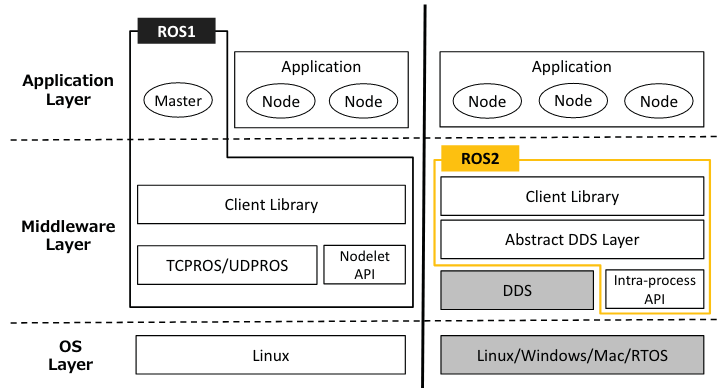
\includegraphics[width=0.95\textwidth]{./figures/ros2-architecture.png}
  \caption{Vergleich der ROS und ROS2 Architektur \cite{maruyamaExploringPerformanceROS22016}}
  \label{fig:ros2-architecture}
\end{figure}

Wie in der Abbildung \ref{fig:ros2-architecture} zu sehen ist, wurde der Master Knoten aus der bisherigen Architektur entfernt. Dies verbessert die Fehleranfälligkeit, da es kein Single Point of Failure mehr gibt. Zusätzlich wurde der Data Distribution Service als Pub/Sub-Mechanismus eingeführt um die Kommunikation zwischen den einzelnen Knoten zu gewährleisten.\\
Die eigentlichen Anwendungen laufen auf eigenständigen Prozessen, die auch als Knoten (\textit{nodes}) bezeichnet werden \cite{maruyamaExploringPerformanceROS22016}. Dies bringt Vorteile wie die der Modularisierung, schnellere unabhängige Entwicklung und die Entkopplung des Systems an ein Zentrales System. Einzelne Knoten können dann über Nachrichten (\textit{messages}) miteinander kommunizieren. Das Austauschen der Nachrichten basiert dabei auf ein Publish/Subscriber Modell, bei dem \textit{topics} zum subscriben oder publishen einer Nachricht nutzt.

% subsubsection ROS 2 (end)

% subsection Robotik Systeme (end)

% >> Subsection of Robotik Systeme
\subsection{Kommunikationsprotokolle} % (fold)
\label{sub:Kommunikationsprotokolle}

Das verwendete Kommunikationsprotokoll ist in der Robotik ein wichtiger Faktor für die Performance und Skalierung der Anwendungen. In \cite{jawharNetworkingMultiRobotSystems2018} wurden dabei verschiedene Protokolle untersucht und bewertet. Wie schon im Abschnitt \ref{sub:Cloud-To-Thing-Continuum} erwähnt, hat man hier jedoch durch die vielen Protokollen einen hohen Aufwand. Die Autoren beschreiben im Paper zusätzlich weitere Hürden die man für Kommunikationsprotokolle im Cloud und Edge Robotics berücksichtigen sollte:

\begin{enumerate}
  \item Die Anzahl der Roboter: Kommunikationsprotokolle müssen bei einer Hohen Anzahl an Robotern skalierbar bleiben und externe Netze unterstützen.
  \item Rechen und Speicherleistung: Je nach Anwendungsfall muss die Rechen und Speicherleistung des Clients berücksichtigt werden. Einfache Roboter zum Beispiel, brauchen ein leichtgewichtiges Protokoll.
  \item Energieeffizienz: Vor allem Roboter nutzen oftmals eine Battery als Energiequelle. Da diese nur eine beschränkte Kapazität haben, sollte Energieeffizienz ein wichtiger Stellenwert im Protokoll haben. Hier wäre es hilfreich, wenn das Protokoll je nach Zustand des Roboters die Energieeffizienz anpassen könnte. Bei Zeitkritischen Anwendungen müssen öfter Netzwerkanfragen gemacht werden als bei einfachen Anwendungen.
  \item Netzwerkdurchsatz: Da man nicht immer mit optimalen Netzen rechnen kann, sollte das Protokoll diese auch unterstützen. Hier müssen vor allem Paketverluste, Störungen und Verzögerungen miteinbezogen werden.
  \item Weiterleitung und Übergabe: Hiermit ist die Weiterleitung und Übergabe von Clients an verschiedene Router zwischen Netzen gemeint. Da Clients, wie zum Beispiel Roboter, sehr beweglich sein können, muss man der Übergang in verschiedene Netze reibungslos laufen können.
\end{enumerate}

Im Fall der Robotik Systeme, ist es wichtig ein simples Protokoll zu haben welches von den meisten Roboter unterstützt wird. Die erste Version von ROS nutzte dabei TCPROS/UDPROS \cite{maruyamaExploringPerformanceROS22016}. Ein auf dem TCP und UDP basiertes Kommunikationsprotokoll. Da dieses, wie schon erwähnt einen zentralen Master Prozess vorausgesetzt hat, ist man für die zweite Version auf den dezentralen \acrlong{dds} umgestiegen. Bei der Nutzung außerhalb der Robotik oder im Kontext des \acrlong{cttc} stößt das \acrlong{dds} jedoch auf seine Grenzen. Die zum aktuellen Zeitpunkt passendste Lösung ist das Zenoh Protokoll.\\
Im folgenden Abschnitt wird zu erst das \acrlong{dds} vorgestellt. Daraufhin wird auf das Zenoh Protokoll, dessen Eigenschaften und Benutzung eingegangen.

\subsubsection{Data Distribution Service} % (fold)
\label{ssub:Data Distribution Service}

Der Data Distribution Service, nachfolgend DDS genannt, ist das Transportprotokoll welches in ROS2 genutzt wird \cite{ConceptsROSDocumentation}. Dieses ermöglicht verschiedene Konfigurationsmöglichkeiten und bietet eine erhöhte Stabilität gegenüber der Kommunikation in ROS. Außerdem abstrahiert es die Schnittstellen für den Nutzer und basiert auf einen verlässlichen Pub/Sub Mechanismus \cite{maruyamaExploringPerformanceROS22016}. Vom \acrlong{dds} gibt es dabei mehrere Implementierungen, so dass es wie eine art Middleware agiert. Man kann also verschiedene DDS Implementierungen nutzen oder diese mit einem externen Protokoll, wie Zenoh, kombinieren.\\
Eine Hauptkomponente von DDS ist die Data-Centric Publish-Subscribe Komponente, nachfolgend DCPS genannt. Diese realisiert den effizienten Datentransport zwischen den heterogenen Prozessen, die alle innerhalb einer gemeinsamen Domäne kommunizieren. Ein wichtiger Bestandteil des DCPS sind die Parametern die man in der Quality-of-Service Policy, nachfolgend QoS genannt, setzen kann. Diese können das Transportverhalten beeinflussen und sind in der offiziellen Spezifikation des Data Distribution Service definiert \cite{DataDistributionService}. Die im Bezug auf die Kommunikation zu den Edge und Cloud Servern relevanten Policies sind in \ref{tab:qos} dargestellt.

\begin{table}
  \caption{DDS QoS Policies\cite{maruyamaExploringPerformanceROS22016}}
  \label{tab:qos}
  \begin{center}
    \begin{tabularx}{\textwidth}{lX}    % Old: \begin{tabular}[c]{l|l}
      \hline
      \multicolumn{1}{c|}{\textbf{Policy}} & 
      \multicolumn{1}{c}{\textbf{Beschreibung}} \\
      \hline
      DEADLINE & Es muss ein Update sowohl auf der Schreib sowie auf der Lese Seite innerhalb eines bestimmten Zeitraumes geschehen. Dies ist besonders hilfreich im Kontext des Durchsatzes um sicher zu gehen, dass die jeweiligen Nachrichten ankommen. \\
      RELIABILITY & Hiermit kann angegeben werden wie zuverlässig die Kommunikation sein muss. Mit der Konfiguration \code{BEST\_EFFORT} werden die Daten am schnellsten gesendet, wobei Teile bei schlechter Verbindung verloren gehen können. Mit der \code{RELIABLE} Option ist die komplette Datenübertragung gesichert. Bei Verlust werden einzelne Datenpakete nachgeschickt. Hier muss man zwischen Sicherheit und Geschwindigkeit abwägen. \\
      DURABILITY & Bei der \code{DURABILITY} Policy kann ein gewisses Caching eingestellt werden, damit später dazukommende Leser in der Message Queue ebenfalls die Nachrichten empfangen können. Dies ist im Hinblick auf den Robotics Use case sehr hilfreich, da man hier durch eine beispielsweise schlechte Konnektivität erst spät eine Verbindung aufbauen kann.\\
      \hline
    \end{tabularx}% 
    % \end{tabular}
\end{center}
\end{table}

% subsubsection Data Distribution Service (end)

\subsubsection{Zenoh} % (fold)
\label{ssub:Zenoh}

Zenoh ist ein Pub/Sub Protokoll, welches ebenfalls die Eigenschaft hat Daten anzufragen oder Operationen auf entfernten Maschinen auszuführen.\\
In Ihrer offiziellen Dokumentation, präsentieren Sie sich als Protokoll mit folgenden Eigenschaften: "[...] protocol unifying data in motion, data at rest and computations"\cite{ZenohZeroOverhead2022}. Damit stellt sich Zenoh als Schlüsseltechnik im Themenbereich des \acrlong{cttc} dar. Das \acrlong{cttc} ist dabei, wie eingangs bereits erwähnt, ein Konzept welches die Möglichkeit beschreibt Ressourcen in Form von Rechenkapazität oder Speicherplatz in einem Kontinuum zwischen einfachen Geräten wie Mikrocontroller oder Robotern hin zur Cloud oder Edge zu nutzen \cite{baldoniZenohbasedDataflowFramework2021}. Für den Cloud und Edge Robotics Bereich ist dieses Konzept sehr interessant, da es viele Themen miteinbezieht, die für die Umsetzung von Anwendungen in dem Bereich relevant sind. Zenoh schließt hier die Brücke zwischen den Robotern und der Cloud, in dem es ein einheitliches Kommunikationsmedium zum Austausch von Daten anbietet. Es müssen also nicht verschiedene Protokolle zwischen den verschiedenen Schichten genutzt werden, sondern Zenoh kann als Ende-Zu-Ende Lösung genutzt werden.

\paragraph{Zenoh Protokoll} % (fold)
\label{par:Zenoh Protokoll}

Die Stärke des Zenoh Protokolls im Vergleich zu anderen Alternativen basiert auf drei Punkten \cite{baldoniZenohbasedDataflowFramework2021}. Zum einen, auf den effizienten Publish/Subscribe Mechanismus welcher unter anderem eine automatische dynamische Suche nach Knoten beinhaltet und Batching der Anfragen unterstützt. Zum anderen, durch die Möglichkeit Daten in geografisch verteilte orten zu speichern, diese gezielt abzufragen. Zuletzt, bietet Zenoh noch eine einfach definierte Semantik um Anfragen zu stellen und verschiedene Aufgaben zu aggregieren.

Zenoh definiert im großen und ganzen 3 Arten von Abstraktionen\cite{ZenohZeroOverhead2022} die wichtig für die Nutzung sind.\\
Die erste grundlegende Abstraktion ist die Darstellung von Ressourcen. Diese werden dabei in Form von Key/Value Paaren dargestellt: \code{(key, value)}. Im Robotics Kontext könnte man hier verschiedene Sensoren und dessen Daten speichern:

\begin{lstlisting}
("robot1/temperature", 23.5)
("robot2/pressure", 1.2)
\end{lstlisting}

Eine weitere wichtige Abstraktion sind Key Expressions. Die Syntax hierfür ist die Key Expressions Language\cite{Eclipsezenoh} und ist in den RFCS des Eclipse Zenoh Projektes dokumentiert. Die wichtigsten beiden Ausdrücke sind die folgenden:

\begin{enumerate}
  \item \code{*} - Dieser Ausdruck entspricht allen Zeichen außer \code{/}. Folgender Ausdruck würde eine Subscription auf die Temperatur Sensoren aller Roboter in der Fabrik 1 und der Robotergruppe A auslösen:\\
    \code{factory1/robotGroupA/*/temperature}
  \item \code{**} - Dieser Ausdruck entspricht allen Zeichen inklusive \code{/}. Folgender Ausdruck würde eine Subscription auf alle Temperatur Sensoren der Fabrik 1 auslösen:\\
    \code{factory1/**/temperature}
\end{enumerate}

Schlussendlich gibt es noch die Abstraktion der Selektoren. Diese erweitern die Key Expressions um Parameter die wie Query-Parameter bei einer URL funktionieren:\\
\code{factory1/robotGroupA/*/temperature?measure=true\&unit=degrees}\\
Wie man also sehen kann, fungieren Selektoren wie URLs ohne Protokoll und Hostname.\\
Selektoren bieten dabei zwei große Anwendungsfälle in Zenoh. Zum einen, können sie verwendet werden um nicht nur nach den Schlüsseln, sondern auch nach dem Wert in einer Anfrage zu filtern. Wenn das Ziel der Zenoh Anfrage das Auslösen einer entfernten RPC-Methode ist, kann man Parameter auch nutzen, um weitere Argumente mitzugeben.

% paragraph Zenoh Protokoll (end)

% subsubsection Zenoh (end)

% subsection Kommunikationsprotokolle (end)



% -------------------------------------------------------------------------------------------------

\section{Realisierung des Cloud-To-Thing Kontinuums} % (fold)
\label{sec:Realisierung des Cloud-To-Thing-Continuums}

Wie im Grundlagen Abschnitt bereits kurz erwähnt, handelt es sich beim \acrlong{cttc} um ein Bestreben, die Nutzung der Ressourcen zwischen Endgeräten und der Cloud in einem Kontinuum zu vereinen. Initiale Ansätze wurden in den letzten Jahren unter anderem von der Eclipse Foundation und dem Unternehmen ADLINK Technology entwickelt \cite{cominardiDevopsEdgeopsVision2021}. Im folgenden Abschnitt, wird das Konzept des \acrlong{cttc} im Kontext der Robotik praktisch betrachtet. Dafür wird die ebenfalls im Grundlagenabschnitt erläuterte Technologie Zenoh und ihre Stärken im Bezug auf das \acrlong{cttc} beleuchtet.

Im Hinblick auf den Robotics Bereich, ist das Protokoll Zenoh sehr Interessant. Wie im Whitepaper zum Thema Edge Computing der Eclipse Foundation \cite{cominardiDevopsEdgeopsVision2021} erwähnt, hilft dieses die Brücke zwischen den einzelnen Komponenten zu schließen. Es tut dies, indem es die Möglichkeit bietet durchgängig das gleiche Protokoll zu Nutzen. Dazu stellt es Schnittstellen in verschiedenen Sprachen bereit \cite{ZenohZeroOverhead2022}. Für Microcontroller und Embedded Devices bietet es Schnittstellen in Rust und C an. Einsteiger können dabei auf die einfacherer Python API zurückgreifen. Um Kompatibilität mit regulären HTTP-Servern zu gewährleisten, bietet Zenoh ein dazugehöriges Plugin an \cite{Eclipsezenoh}. Dieses bildet Zenoh-Pfade auf URLs ab. In Situationen, in denen ein Web Server existiert der auf Datenbanken zugreift, kann dieser Ansatz hilfreich sein. Für diese Seminararbeit von Interesse und im Folgenden näher betrachtet, ist das Zenoh Plugin für den \acrlong{dds}. Dieses ermöglicht die Integration mit Roboter die das ROS2 Betriebssystem nutzen \cite{Eclipsezenoh}. Zusammengefasst, kann man Zenoh nutzen, um zum Beispielsweise im Robotics Bereich einen direkten Zugang zu Edge und Cloud Services zu ermöglichen.\\

Ein einfaches Beispiel welches die Essenz des \acrlong{cttc} zeigt, ist die Nutzung von Sensordaten im industriellen Kontext. Zur besseren Veranschaulichung, wird das Konzept des \acrlong{cttc} anhand eines vereinfachten Beispiels dargestellt. Dieses enthält einen beweglichen Roboter, einen Steuerungsserver und eine logging Datenbank:

\begin{figure}
  \begin{center}
    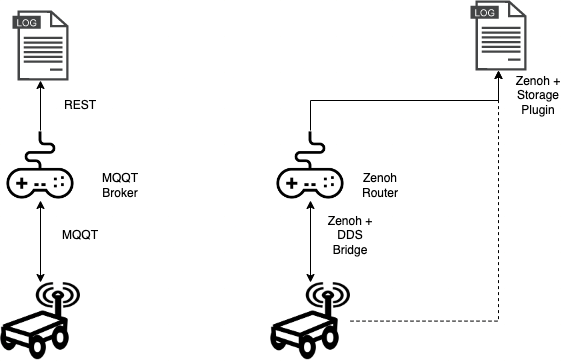
\includegraphics[width=0.5\textwidth]{./figures/cttc_demo.png}
  \end{center}
  \caption{Vereinfachtes Beispiel zur Erklärung des \acrlong{cttc}}
  \label{fig:cttc_demo}
\end{figure}

In Abbildung \ref{fig:cttc_demo} ist die zuvor beschriebene vereinfachte Architektur mit den jeweiligen Kommunikationsprotokollen dargestellt. Auf der linken Seite wird dabei MQQT für die Verbindung zwischen Roboter und Steuerungsserver genutzt. Um die Daten auf der logging Datenbank zu hinterlegen, wird eine POST-Anfrage auf eine REST-Schnittstelle getätigt.\\
Aus Sicht des vom \acrlong{cttc} angestrebten Kontinuums, ist diese Architektur nicht optimal. Durch die verschiedenen Kommunikationsprotokolle kommt es zu Unterbrechungen im Informationsfluss. Dies erhöht die Latenz sowie die Fehlerwahrscheinlichkeit durch wechselnden Technologien. Der Roboter hätte in diesem Fall auch keine Möglichkeit auf direktem Wege die logging Datenbank anzusprechen und müsste über eine Schnittstelle im Routing Server gehen. Eine Ende-Zu-Ende Kommunikation ist also nicht möglich. Dazu kommen die Eigenschaften der eingesetzten Technologien. Das MQQT-Protokoll \cite{enwiki:1127334174} wurde eingangs nicht für den Einsatz in heterogenen Umgebungen oder für die Skalierung im Zeitalter des Cloud Computings erstellt. Dazu kommt, dass die meisten MQQT-Architekturen einen Nachrichten-Broker voraussetzen und Peer-To-Peer Modelle nicht sehr häufig genutzt werden.\\

Im Vergleich zu der traditionellen Architektur, befindet sich auf der rechten Seite eine Alternative auf Basis von Zenoh die den \acrlong{cttc} Ansatz verfolgt. Zwischen dem Roboter und dem Steuerungsserver wird dabei Zenoh und eine DDS-Bridge\cite{Eclipsezenoh} genutzt. Die DDS-Bridge dient zur Übersetzung der Nachrichten vom \acrlong{dds}. Die Funktionsweise dieser wird dabei im nächsten Abschnitt \ref{sec:Integration von ROS2 mit Zenoh} näher erläutert. Für die Einbindung der logging Datenbank, kann man eine von den eingangs erwähnten Zenoh Erweiterungen nutzen die eine Schnittstelle für die externe Datenbank bietet. Es wäre hier ebenfalls möglich, über eine direkte Verbindung Nachrichten vom Roboter an die logging Datenbank zu verschicken. Eine ausführlichere Erklärung einer Peer-To-Peer Architektur wird in Abschnitt \ref{sec:Cloud und Edge Robotic Use cases} behandelt.\\
Wie man an dem Vergleich erkennen kann, erfüllt die zweite Architektur die Ansätze des \acrlong{cttc} besser als die erste. Es wird dabei eine transparente Kommunikationsstruktur ermöglicht die unabhängig von der jeweiligen Lage der Komponente erreichbar ist. Eine Skalierung in Form von weiteren Servern oder Robotern wäre hier ebenfalls einfach möglich.

% section Realisierung des Cloud-To-Thing-Continuums (end)


\section{Integration von ROS2 mit Zenoh} % (fold)
\label{sec:Integration von ROS2 mit Zenoh}

Wie im vorangegangenen Abschnitt beleuchtet, ist Zenoh ein wichtiger Baustein um die Brücke im \acrlong{cttc} zu schließen. Es nimmt die Rolle des Transportprotokolls für alle Teilnehmer im Kontinuum ein. Aus diesem Grund macht es Sinn, Zenoh in ROS2 einzubinden um die Roboter in das Kontinuum zu integrieren.\\
Aus dieser Motivation heraus, wird in diesem Abschnitt die Integration von ROS2 mit Zenoh erläutert. Dabei wird zu Beginn auf die generellen Gründe hinter der Nutzung von Zenoh im Robotics Bereich eingegangen. Schließlich, wird die Technische Implementation beschrieben und die Nutzung im \acrlong{cttc} erläutert.\\

Die Nutzung von Zenoh in ROS2 hat viele positive Auswirkungen auf die Kommunikation zwischen den Robotern. Neben der bereits erwähnten Einbindung in das \acrlong{cttc}, bietet Zenoh eine Reihe von Vorteilen gegenüber dem standard Kommunikationsservice in ROS2, dem \acrlong{dds}.\\

Ein Hauptgrund Zenoh zu nutzen ist das ineffiziente Discovery Protokoll vom \acrlong{dds}. Dieses wurde mit kabelgebundenen Architekturen im Hinterkopf entworfen und kommt bei modernen Kabellosen Architekturen an ihre Grenzen. Erkennen lässt es sich am großen overhead, welches das DDS Discovery Protokoll im Vergleich zu Zenoh im Netzwerk erzeugt \cite{ZenohZeroOverhead2022}. Der Grund für die Ineffizienz beim austauschen der Daten ist die Funktionsweise des Discovery Mechanismus. Bei einem falsch konfigurierten Netz sendet der Discovery Mechanismus dabei immer weitere Suchanfragen aus und kann das Netz massiv überlasten. ROS2 ging dieses Problem an, in dem es einen neuen Discovery Server \cite{DiscoveryServerSettings} einführte der das Netzwerk Overhead verringert. Doch wie im Namen enthalten, wird hier ein neuer, zentraler Server gebraucht der die Discovery unterstützt. Dies macht es wiederrum für viele Peer-To-Peer Anwendungsfälle schwer nutzbar. Zenoh wiederrum, bietet ohne zentralen Server ebenfalls eine gute Discovery Performance. Im Gegensatz zu dem Discovery Mechanismus in DDS, nutzt Zenoh das Konzept der "Resource Generalisation"\cite{ZenohZeroOverhead2022}. Dabei kann das Protokoll je nach Einstellung nur ein Bruchteil der Daten übertragen die vom Netzwerk für die Entdeckung der Services gebraucht werden. Bei einem Roboter der folgende Datenquellen published:
\begin{enumerate}
  \item Temperatur: \code{/robot1/sensor/temperatue}
  \item Druck: \code{/robot1/sensor/pressure}
  \item Orientierung: \code{/robot1/dynamics/odometry}
\end{enumerate}

Kann der Zenoh Router 'Ressource Generalisation' anwenden, in dem es nur die Daten \code{/robot1/sensor/**} und \code{/robot1/dynamics/**} oder \code{/,robot1/**} im Discovery Mechanismus weitergibt. Dadurch kann die Datenmenge in einer Anfrage komprimiert werden und das Netzwerk besser skalieren. Dies ist wichtig , wenn man beispielsweise über das Internet mit sehr vielen Clients skalieren möchte.\\
Das Zweite Argument für die Nutzung von Zenoh als Kommunikationsprotokoll ist die Skalierbarkeit im Bezug auf das \acrlong{cttc}. Das Ziel ist wie im Eingangskapitel erwähnt, die Skalierung auf Ebene des Internets. Durch den bereits erwähnten Discovery Mechanismus von DDS, stößt man hier jedoch an Grenzen. Neben dem bereits erwähnten Problem des Netzwerk Overheads, bringt es weitere Nachteile im Kontext der Skalierung mit. Roboter die sich in weiteren Subnetzen befinden, können nicht automatisch gefunden werden. Daraus ergibt sich ein Problem wenn man über das Internet Skalieren möchte. Da vor allem letzteres ein wichtiger Grundpfeiler beim \acrlong{cttc} ist, lohnt es sich eine Integration mit Zenoh einzubauen.\\

Außer den genannten Gründen, macht die Unterstützung von leistungsschwachen Robotern in einem Umfeld instabiler Verbindungen das Zenoh Protokoll interessant für die Robotik. Zum einen braucht man keine Rücksicht auf die Leistung verschiedener Roboter nehmen und kann sich auf den jeweiligen Use case konzentrieren den man erreichen möchte. Zum anderen kann Zenoh mit instabilen Verbindungen gut umgehen. Grund dafür ist die Konstruktion der Verbindungen zwischen den Teilnehmern in einem Zenoh Netzwerk. Dabei werden bei einer Zenoh Verbindung zwei Arten von Kanälen aufgebaut \cite{Eclipsezenoh}. Der eine Kanal ist auf Zuverlässigkeit getrimmt. Der andere arbeitet nach dem \textit{Best Effort} Prinzip und kann nicht zwangsläufig eine fehlerfreie Übermittlung garantieren. Dabei ist es möglich zuverlässige Kanäle zwischen zwei Teilnehmern zu erstellen die mehrere Hops dazwischen haben. Das ist Sinnvoll, wenn die Zuverlässigkeit eine hohe Priorität hat. Zusätzlich kümmert sich das Protokoll um die Fragmentierung und die maximale Nutzung der vorhandenen Verbindung um möglichst effizient zu arbeiten.\\

Zusammenfassend ist die Einbindung von Zenoh in ROS2 eine große Hilfe um die Robotik mit den Zielen des \acrlong{cttc} zu vereinen und das in \ref{sub:Cloud-To-Thing-Continuum} vorgestellte Konzept des Robot-to-anything (R2X) zu erreichen. Es tut dies, in dem es viele Defizite von DDS ausgleicht und die Skalierbarkeit entlang des \acrlong{cttc} möglich macht.\\

\subsection{Einbindung von Zenoh im Data Distribution Service} % (fold)
\label{sub:Einbindung von Zenoh im Data Distribution Service}

Nachdem die Motivation für die Nutzung von Zenoh in ROS2 erläutert wurde, wird nun auf die technische Implementierung eingegangen. Diese basiert auf einen leichtgewichtigen Übersetzer zwischen dem ROS2 Roboter und einem weiteren Zenoh Client. Das Ziel ist dabei die transparente Überführung von DDS-Nachrichten in einen für das Zenoh Protokoll geeignetes Format. Mit diesem, ist es dann möglich Nachrichten zwischen verschiedenen Zenoh Knoten auszutauschen. Diese können weitere ROS2 Instanzen oder Server an der Edge oder Cloud sein.\\

Um externe Services an Zenoh anzubinden werden Plugins genutzt. Diese bilden die Brücke zwischen den verschiedenen Systemen. Im Fall von ROS2 wird eine Brücke zwischen dem \acrlong{dds} und dem Zenoh Protokoll gebraucht. Das Zenoh DDS Plugin erfüllt diese Aufgabe und ist als Open Source Projekt auf GitHub zu finden \cite{Eclipsezenoh}.\\
Um Nachrichten an das Zenoh Protokoll weiterzuleiten, erkennt das Plugin die vom \acrlong{dds} bereitgestellten Entities und generiert ein jeweiliges Paar für Zenoh.

\begin{figure}
  \begin{center}
    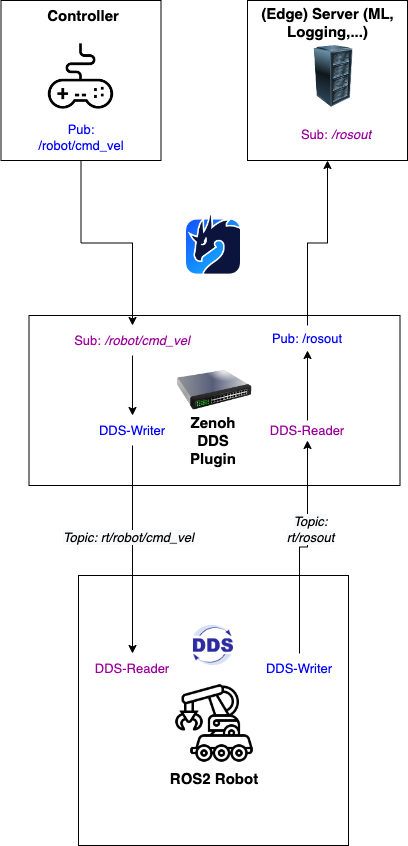
\includegraphics[width=0.5\textwidth]{figures/ros2-dds.drawio.png}
  \end{center}
  \caption{ROS2 DDS Plugin}
  \label{fig:ros2-dds}
\end{figure}

Das Beispiel in Abbildung \ref{fig:ros2-dds} zeigt die Funktionsweise in einer vereinfachten Form. Auf dem ROS2 Roboter gibt es dabei ein DDS-Reader und ein DDS-Writer. Der Reader hört auf das Topic \code{rt/robot/cmd\_vel} und bekommt hier Informationen um seine Geschwindigkeit anzupassen. Der DDS-Writer published dabei allgemeine ROS Informationen auf dem Topic \code{rt/rosout}.\\
Um das Zenoh Protokoll anzubinden kommt jetzt das Zenoh DDS Plugin zum Einsatz. Dieses findet automatisch die vom DDS Angebotenen Reader und Writer. Daraufhin erstellt er für jeden der Topics einen dazugehörigen DDS-Reader oder Writer. Für einen Reader, einen Writer und umgekehrt. Dies lässt sich an \ref{fig:ros2-dds} in der ersten Verbindung erkennen. Nützlich ist auch, dass das Plugin die in \ref{sub:Einbindung von Zenoh im Data Distribution Service} angesprochenen Quality-of-Service Policies ebenfalls übernimmt. Schlussendlich erstellt das Plugin für jeden Reader einen Zenoh Subscriber und für jeden Writer einen Zenoh Publisher mit dem der Roboter nun an das Zenoh Netzwerk eingebunden wäre. In dem betrachteten Beispiel gibt es noch einen Controller der die Robotersteuerung übernimmt und ein Server der die Log Daten aus dem Roboter speichert.

% subsection Einbindung von Zenoh im \acrlong{dds} (end)

% section sec:Integration von ROS2 mit Zenoh (end)


\section{Cloud und Edge Robotic Architekturen} % (fold)
\label{sec:Cloud und Edge Robotic Architekturen}

Die Nutzung von Cloud und Edge Computing Ressourcen in Kombination mit Robotern öffnet die Möglichkeit für verschiedene Arten von Architekturen. Neben der einfachen Kommunikation zwischen Robotern, ermöglichen Edge und Cloud Server komplexere Systeme die zum Beispiel bei dem effizienteren Auslagern von Ressourcen genutzt werden können. Vor allem Dezentralisierte Architekturen sind diesbezüglich interessant. Roboter können dabei die Speicherung von Daten oder Ausführung von Rechenleistung an einem anderen Knoten in einem System auslagern. In \cite{jawharNetworkingMultiRobotSystems2018} beschreibt Imad Jawhar et al. verschiedene Architekturen die sich im Speziellen auf Multi Roboter Systeme beziehen. Dabei nennt er vier Architekturen:

\begin{enumerate}
  \item Zentralisierte: Hier gibt es einen Zentralen Knoten der alle Clients verwaltet. Problem hierbei ist ganz klar der Single point of failure und die Skalierung.
    \item Hierarchische: Bei dieser Art der Architektur gibt es mehrere übergeordnete Steuerungsknoten. Dieses Konzept kann man näherungsweise mit einer Edge Architektur vergleichen. Der Vorteil von dieser Architektur ist die Skalierung. Beim hinzufügen von Robotern können weitere Instanzen, Beispielweise im Edge, hinzugefügt werden. Nachteil ist die Zuverlässigkeit, da insgesamt mehr Instanzen involviert sind.
      \item Dezentralisiert: Wie eingangs Erwähnt hat man hier keine zentrale Instanz. Dadurch ist das System sehr robust, jedoch auf Kosten der Synchronisation die komplexer ist.
        \item Hybrid: Nach den Autoren des Papers, ist dies in Multi Roboter Systemen die Populärste Alternative. Dabei kombiniert man verschiedene der oben genannten Architekturen um eine gute Balance zwischen der Skalierbarkeit von dezentralisierten und der Zuverlässigkeit von zentraleren Modellen.
\end{enumerate}

Im folgenden werden verschiedene Arten von Netzwerk Teilnehmern und deren Eigenschaften in einem Cloud und Edge Robotics Netzwerk beschrieben. Darauf aufbauend, werden dann drei Arten von Architekturen für Cloud und Edge Robotics erläutert und jeweils die Anwendung im Transportprotokoll Zenoh erläutert.\\

Die erste Art von von Teilnehmer ist ein einfacher Client. Dieser dient als Endanwender im System. Er kann auf Topics im Netzwerk subscriben oder selber Daten publishen. Im Gegensatz zu den weiteren Teilnehmern, kann ein Client kein Routing vornehmen. Im Kontext dieser Arbeit, ist ein Roboter oder Microcontroller ein Beispiel für ein Client. Dieser sendet Umgebungsdaten und Sensordaten aus und bekommt Steuerungsbefehle aus dem Netzwerk. In Zenoh können Clients auf verschiedenster Weise Implementiert werden. Dafür bietet Zenoh verschiedene Client Bibliotheken an. Beispielsweise für Rust, Python oder C. Speziell ist ebenfalls die Pico Client Bibliothek, die es ermöglicht sehr leistungsschwache Geräte zu unterstützen.\\
Im Gegensatz zum Client steht der Router. Dieser ist ausschließlich für die Weiterleitung von Daten und Befehlen zuständig und hat keine Rolle als Anwendung. Zenoh bietet hierfür ein Kommandozeilentool(\code{zenohd}) an welches unter anderem für verschiedene Plattformen als einfache Binäre Datei zur Verfügung steht. Der Zenoh Router lässt sich dabei leicht mittels Kommandozeilenparameter oder einer Konfigurationsdatei für den jeweiligen Use Case anpassen. Ein Beispiel hierfür sind die Anbindungen an Datenbanken oder andere Speichermöglichkeiten. Damit ist es möglich, neben den bekannten Publish/Subscribe Funktionalitäten, Daten per \code{PUT} Query abzuspeichern.\\
Schlussendlich gibt es noch sogenannte Peers. Diese stellen eine Mischung aus Client und Router dar. Das heißt, dass sie sowohl Anwendungs als auch Routing Fähigkeiten haben. Bekannt sind Peers aus dem Peer-to-Peer Netzwerkmodell. In Zenoh lässt sich ein Peer aus der Nutzung von einer Client Bibliothek und dem Zenoh Router nutzen. Beispielsweise könnte ein leistungsstarker Cloud Server Nachrichten sowohl Routen als auch die im Zenoh Speicher abgelegten Daten direkt zu Weiterverarbeitung in einem Machine Learning Model nutzen.\\

Bei den Netzwerk Architekturen gibt es im Cloud und Edge Bereich auch drei große Kategorien. Peer-to-Peer Netze, Router und Broker basierte Architekturen.\\
Die erste Art von Architekturen sind Peer-to-Peer Netze \cite{schollmeierDefinitionPeertoPeerNetworking2001}. Diese nutzen Peers um miteinander zu kommunizieren. Im Cloud und Edge Computing Bereich, könnte man diese als Server darstellen die jeweils eine Aufgabe ausführen und miteinander kommunizieren. Hier wäre eine Kombination zwischen Rechnern an der Edge und in der Cloud vorstellbar. Die Anwendung könnte hier Beispielweise die Auswertung der Daten im Edge Server und die weiterverarbeitung in einer Leistungsstärkeren Cloud Instanz sein. Spezialfälle von Peer-to-Peer Netzwerke sind Mesh \cite{cilfoneWirelessMeshNetworking2019} und Clique \cite{enwiki:1096684789} Netzwerke. Erstere charakterisieren sich dadurch, dass sie zusammenhängend sind. Man kann also von jedem Knoten, jeden anderen Knoten erreichen. Falls keine direkte Verbindung existiert, kann dafür auch ein Umweg über einen weiteren Knoten genommen werden. Bei Clique Peer-to-Peer Netzwerke, hat jeder Knoten eine Verbindung zu jedem anderen Knoten. Dies kann man dann ausnutzen und die direkten Verbindungen zwischen den Peers ausnutzen. Zenoh unterstützt dank dem dynamischen discovery Mechanismus automatisch alle Arten von Peer-to-Peer Typologie.\\
Router basierte Architekturen sind die zweite Art von Architekturen. Hier stehen Router im Vordergrund um Nachrichten zwischen verschiedenen Clients und Peers auszutauschen. Wie im Use Case \ref{sub:Steuerung über WAN (Internet)} zu sehen, eignet sich diese Art der Architektur gut für die Skalierung über weit entfernte Netze. Beispielsweise über das Internet. Nachrichten können auch über mehrere Router weitergeleitet werden. Dies ist in Abbildung \ref{fig:Cloud und Edge Robotics Architekturen} der Fall. Hier ist ein Client mit jeweils einem eigenen Router verbunden. Um Nachrichten von einem Client zum anderen austauschen zu können, müssen diese über beide Router geleitet werden.\\
Das letzte relevante Architektur Muster im Cloud und Edge Robotics Bereich ist der Broker basierte Ansatz. Dieser ist aus Message Queues wie RabbitMQ \cite{AMQP091Model} bekannt und ähnelt der Router basierten Architektur. In diesem Fall sind aber alle Clients mit dem gleichen Router verbunden. Das heißt, dass alle Clients diesen nutzen müssen um Nachrichten auszutauschen. Im Falle einer Roboterflotte kann ein zentraler Broker eine gute Idee sein. Nachrichten können dann Zentral weitergeleitet werden und Konflikte sind einfacher vorzubeugen.\\

\begin{figure}
  \begin{center}
    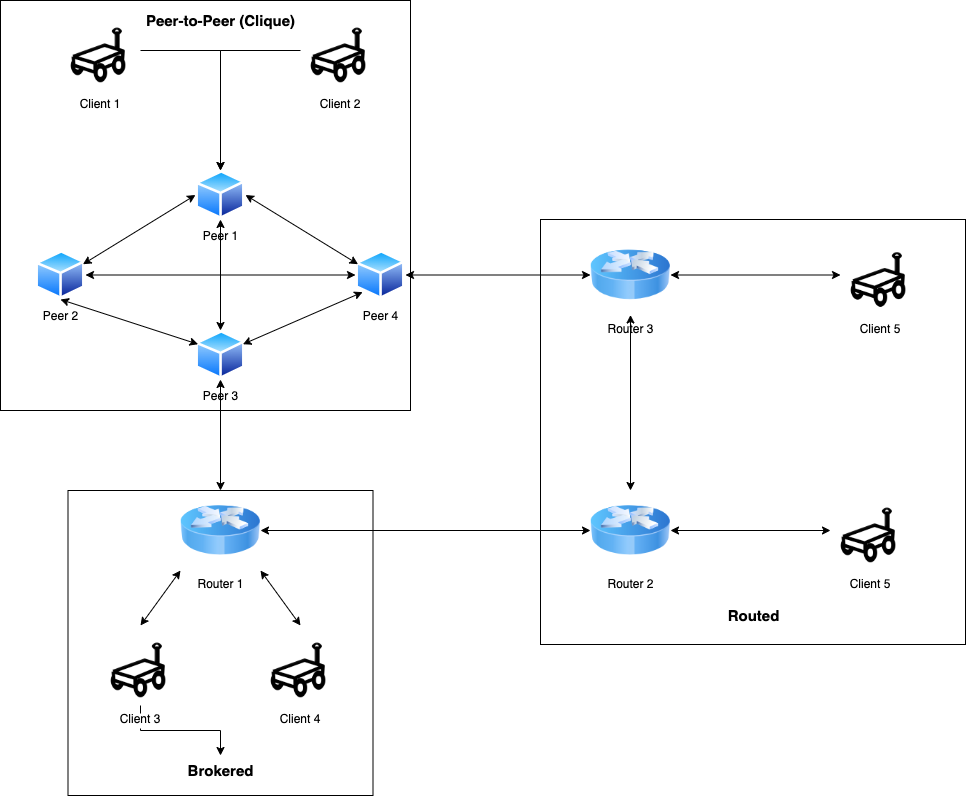
\includegraphics[width=0.8\textwidth]{figures/topologies.drawio.png}
  \end{center}
  \caption{Cloud und Edge Robotics Architekturen}
  \label{fig:Cloud und Edge Robotics Architekturen}
\end{figure}

In \ref{fig:Cloud und Edge Robotics Architekturen} sind die die drei zuvor beschriebenen Architekturen mit den jeweiligen Teilnehmern dargestellt. Oben Links ist die Peer-to-Peer Architektur mit dem Sonderfall einer Clique dargestellt. Diese beinhaltet ebenfalls einen Broker basierten Teil, da \textit{Client 1} und \textit{Client 2} jeweils über \textit{Peer 1} gehen müssen um miteinander zu kommunizieren. Rechts davon befindet sich eine Router basierte Architektur, wie auch im oberen Abschnitt beschrieben. Beide \textit{Clients 5/6} müssen jeweils über Ihre eigenen Router gehen um mit anderen Teilnehmern zu kommunizieren. Schlussendlich ist im unteren Bereich wieder eine Broker basierte Architektur abgebildet wie sie zuvor schon beschrieben wurde.

% section Cloud und Edge Robotic Architekturen (end)


\section{Cloud und Edge Robotic Use Cases} % (fold)
\label{sec:Cloud und Edge Robotic Use cases}

Nachdem in den vorangegangenen Abschnitten relevante Technologien und Architekturen rund um das Thema Cloud und Edge Robotics vorgestellt wurden, wird im folgenden auf verschiedene Use Cases eingegangen und wie man sie mit den bereits besprochenen Konzepten realisieren kann. Dabei werden Konzepte wie die der digitalen Zwillinge, dem Nutzen von verschiedenen Schnittstellen oder dem Zugang über entfernte Systeme behandelt die bereits im Cloud und Edge Computing so wie Robotics Bereich eine Rolle spielen.\\

\subsection{Digitale Zwillinge in der Robotik} % (fold)
\label{sub:Digitale Zwillinge in der Robotik}

Das Konzept der digitalen Zwillinge beschreibt die Möglichkeit, virtuelle Abbilder von Objekten aus der physischen Welt zu erzeugen und für verschiedenen Anwendungszwecke zu nutzen \cite{fullerDigitalTwinEnabling2020}. Beispiele hierfür sind das Testen von Software, der Einsatz von Simulationen oder die Leistung im Vorhinein zu verbessern.\\
Die Robotik ist ein interessanter Bereich wenn es um die Anwendung von digitale Zwillingen geht. Roboter können dabei zum Beispiel digital repliziert werden und so einfacher getestet oder gesteuert werden. Im folgenden Use Case, wird eine im Vorhinein aufgenommene Sequenz an Aktionen in einer Datenbank gespeichert. Es wird also eine Simulation der Aktionen die ein Roboter ausführt zuvor aufgenommen um später auf einem oder mehreren Roboter ausgespielt zu werden. Dies kann vor allem in der Industrie nützlich sein, wenn man eine Kontrollierte Umgebung hat die keine externe Faktoren hat die eine Simulation stören könnte. Unternehmen könnten hiermit einzelne oder mehrere Roboter in einer Fabrik automatisiert jederzeit auf eine bestimmte Sequenz von Aufgaben ansetzen und Fehler der Roboter durch weitere Simulation verbessern.\\

Der Aufbau des Use Cases ist in \ref{fig:Digitale Zwillinge in der Robotik} dargestellt. Dafür werden folgende Komponenten benötigt:

\begin{enumerate}
  \item Simulator: Mit diesem ist es möglich, die Aktionen eines Roboters zu simulieren und aufzunehmen. Dieser veröffentlicht die Simulationsdaten an den Zenoh Router. Der Simulator verhält sich dabei wie ein ROS2 System. Aus diesem Grund wird hier noch das Zenoh DDS Plugin genutzt.
  \item Zenoh Router: Um die Daten zwischen den verschiedenen Komponenten auszutauschen und weiterzuleiten wird das Zenoh Protokoll verwendet. Dafür wird ein zentraler Zenoh Router in der Cloud eingesetzt. Dieser nimmt die Daten des Simulators an, leitet eine Speicherung in der Datenbank ein und veröffentlicht diese an einem späteren Zeitpunkt an den Roboter.
  \item Datenbank: In dieser werden die Aktionen gespeichert, die im Roboter eingespielt werden sollen. Diese können zum Beispiel durch das Influx Datenbank Plugin für Zenoh angebunden werden. Influx ist dabei eine ein Datenbank Managementsystem welches auf das speichern von Zeitreihen spezialisiert ist. Dies ist hilfreich, um beim Abrufen der Simulation die Daten in der richtigen Reihenfolge auszugeben. Interessant ist hier ebenfalls die Einbindung mit Zenoh. Wie bei der Beschreibung der Router in Abschnitt \ref{sec:Cloud und Edge Robotic Architekturen} angedeutet, kann man die Datenbank durch ein Zenoh Plugin direkt mit dem Zenoh Router verbinden. Daraufhin ist es dann möglich, alle zu einem Topic (In diesem Fall \code{robot1/rt/cmd\_vel}) gehörenden Daten automatisch in der Datenbank über den Router zu speichern.
  \item Edge Server und Roboter: Um das einspielen der Simulation in den realen Roboter zu ermöglichen, wird ein Edge Server eingesetzt. Wenn die Simulation im Roboter eingespielt werden soll, startet dieser eine Query auf das \code{robot1/rt/cmd\_vel} Topic. Dies löst eine Anfrage in der Datenbank aus, welche die Daten aussendet. Der Edge Server published diese dann nur noch an den Roboter der auf diese subscribed und die Aktionen ausführt.
\end{enumerate}

\begin{figure}
  \begin{center}
    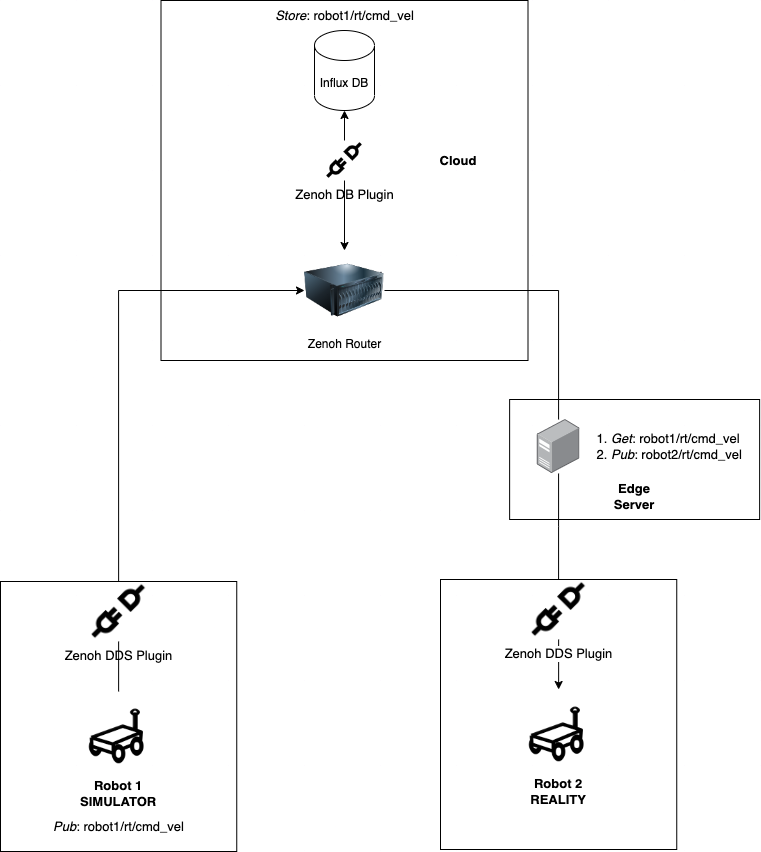
\includegraphics[width=0.6\textwidth]{figures/digitalle-zwillinge.drawio.png}
  \end{center}
  \caption{Digitale Zwillinge in der Robotik}
  \label{fig:Digitale Zwillinge in der Robotik}
\end{figure}

% subsection Digitale Zwillinge in der Robotik (end)

\subsection{Robotersteuerung über den Browser} % (fold)
\label{sub:Robotersteuerung über den Browser}

Die Telerobotik ist ein Teilgebiet der Robotik, bei der es um die Steuerung von Robotern aus der Ferne geht \cite{.mMotionControlArtificial2018}. Dies kann von Vorteil sein, wenn Roboter in einer gefährlichen Umgebung eingesetzt werden oder zentral gesteuert werden sollen. Beispiele hierfür sind Roboter die mit radioaktiven Stoffen arbeiten oder welche die medizinische Operationen aus der Ferne ermöglichen. Vor allem durch die immer besser werdenden Internetverbindungen rückt dieser Use Case wieder in den Vordergrund. Durch die besseren Verbindungen, verringern sich die Latenzzeiten, die wiederrum das entfernte steuern der Robotern erleichtern. Dazu kommen die heutzutage weit verbreiteten Steuerungsschnittstellen wie die der Maus, Tastatur oder Bildschirm. Mit diesen ist es heutzutage nahezu jedem möglich einen Roboter ohne spezielle Hardware zu steuern. In diesem Abschnitt wird ein relativ einfacher Use Case beschrieben der sich mit der Telerobotik beschäftigt. Dabei wird ein Roboter mit Hilfe eines Web Browsers gesteuert.\\

Für den Telerobotik Use Case werden folgende Komponenten benötigt:

\begin{enumerate}
  \item Roboter: Dieser nutzt wie im letzten Use Case das Zenoh DDS Plugin um mit dem Zenoh Protokoll zu kommunizieren und ist mit einem Zenoh Router in der Cloud verbunden.
  \item Zenoh Router: Dieser läuft auf einem Server in der Cloud und bindet das Zenoh REST Plugin ein.
  \item Zenoh REST Plugin: Bietet eine REST-Schnittstelle um Anfragen von HTTP Clients entgegen zu nehmen. Es nutzt dafür die im Netzwerk bekannten Schlüsseln aus den Anfragen, die dann zur Abfrage genutzt werden können. Um Nachrichten vom Roboter an den Web Client zu schicken, werden Server-Sent Events genutzt die Nativ als Web Schnittstelle im Browser vorhanden ist.
  \item Browser: Enthält ein einfaches Programm zur Steuerung des Roboters, kommuniziert per HTTP mit dem Zenoh REST Plugin und bekommt die Informationen durch die erwähnten Server-Sent Events.
\end{enumerate}

\begin{figure}
  \begin{center}
    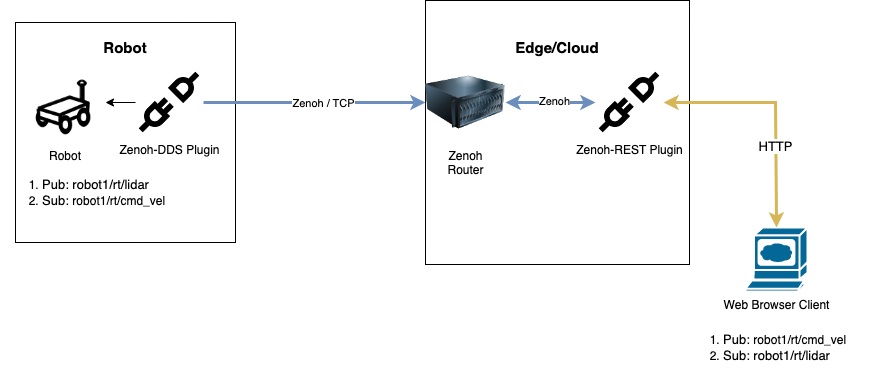
\includegraphics[width=0.95\textwidth]{figures/remote-steuerung.drawio.png}
  \end{center}
  \caption{Robotersteuerung über den Browser}
  \label{fig:Robotersteuerung über den Browser}
\end{figure}

Im vorangegangenen Beispiel sendet der Roboter die Bewegungsdaten über das Topic \code{robot1/rt/lidar} an den den Web Client. Dieser kann die Daten auswerten und darauf über das Topic \code{robot1/rt/cmd\_vel} die Geschwindigkeit anpassen.
Wie man also in \ref{fig:Robotersteuerung über den Browser} erkennen kann, ist die Einbindung von externen Clients mittels dem REST-Protokoll relativ einfach. Dies eröffnet eine weitreichende Möglichkeiten um weitere Endgeräte wie zum Beispiel Smartphones an das \acrlong{cttc} anzubinden.

% subsection Robotersteuerung über den Browser (end)

\subsection{Steuerung über WAN (Internet)} % (fold)
\label{sub:Steuerung über WAN (Internet)}

Entfernte Zugriffe auf Roboter sind wie im letzten Kapitel beschrieben ein wichtiger Use Case für die Robotik. Oftmals sind die Gegebenheiten des Netzwerkes jedoch nicht so optimal wie im vorhergegangenen Beispiel. Vor allem im Bereich des Edge und Cloud Computing muss eine Nachricht verschiedene Netze durchqueren um von einem Sender zu einem Empfänger zu gelangen. Um verschiedene Netze zu durchqueren wird oftmals eine Netzwerk Adressübersetzung, kurz NAT, eingesetzt. Um trotz der verschiedenen Netzüberquerungen einen einfachen Zugriff auf die Roboter zu ermöglichen, muss das genutzte Protokoll diese Gegebenheiten berücksichtigen.\\
Im Folgenden Use Case wird wieder eine entfernte Steuerung eines Roboters beschrieben. Hierbei wird der Fokus jedoch auf die Überbrückung der verschiedenen Netze gelegt.\\

Der Aufbau dieses Use Cases ist von den Komponenten ähnlich wie die beiden vorherigen. Die Steuerung wird in dem Beispiel abstrahiert.\\
Das Ziel an diesem Beispiel ist es einen Roboter von einem entfernten Netzwerk aus zu steuern. Dieses kann sich zum Beispiel geographisch an einem anderen Ort befinden. In \ref{fig:Steuerung über WAN (Internet)} werden zwei Möglichkeiten zur Verbindung betrachtet.\\
Bei der ersten Verbindung handelt es sich um die durchgehende Linie in \ref{fig:Steuerung über WAN (Internet)}. In diesem Fall kann das Netzwerk des Roboters keinen öffentlichen Port, wie zum Beispiel für eine TCP Verbindung öffentlich zur Verfügung stellen. Man braucht also einen externen Server bei der man eine Subscription erstellen kann. Wie in der Abbildung zu sehen, wird dies mit einem einfachen Cloud Server gelöst. Auf diesem läuft ein Zenoh Router, der durch eine öffentliche Adresse zugänglich ist. Sowohl die Steuerung als auch das Zenoh DDS Plugin können dann eine Verbindung mit dem Router im Cloud Server aufbauen. Diese Lösung ist für Anwendungen interessant bei denen man keinen Einfluss auf das Netzwerk hat oder dieses aus Sicherheitsgründen nicht ändern kann.\\
Die Alternative, direkte Verbindung, wird als gestrichene Linie dargestellt. Im Netzwerk des Roboters wird dabei ein Port für die TCP Verbindung geöffnet und die eingehenden Anfragen an das DDS Zenoh Plugin weitergeleitet. Die Steuerung kann dann eine direkte Verbindung zum Plugin aufbauen.\\

\begin{figure}
  \begin{center}
    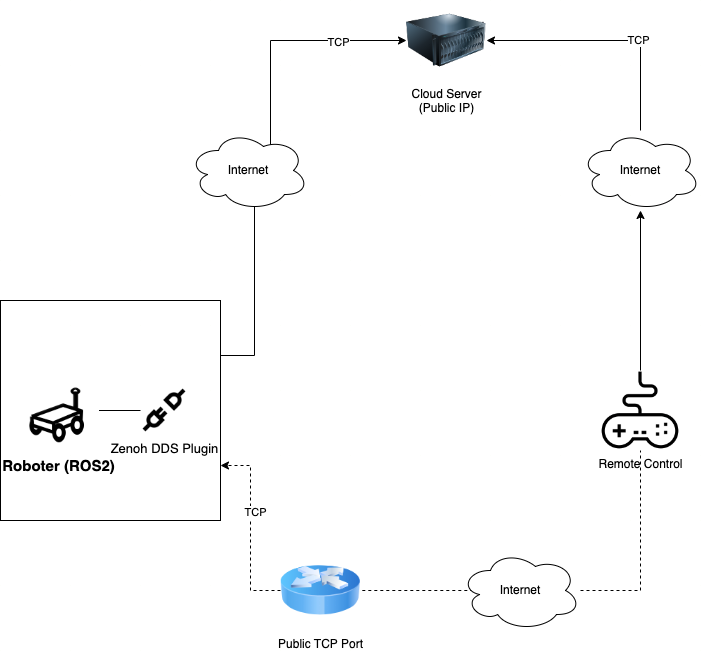
\includegraphics[width=0.6\textwidth]{figures/wan-steuerung.drawio.png}
  \end{center}
  \caption{Steuerung über WAN (Internet)}
  \label{fig:Steuerung über WAN (Internet)}
\end{figure}

Eine wichtige Funktion von verteilten Systemen ist die Ausfallsicherheit. Um dies im oberen Beispiel zu gewährleisten, kann man einen zweiten Zenoh Router in einer weiteren Cloud Instanz einrichten. Diese wird mit der ersten Instanz verbunden. Als Verbindungsparameter werden für die Steuerung und dem Zenoh DDS Router die Adressen beider Server mitgegeben. Im Falle des Ausfalls von einem Server, schalten beide Clients automatisch auf den zweiten Router um.\\
Anhand des letzten Beispiels, kann man eine weitere nützliche Eigenschaft für das \acrlong{cttc} erkennen. Mit Zenoh wird eine Möglichkeit geboten, verschiedene Akteure mittels verschiedenen Protokollen, an geographisch verteilten Orten zu Verbinden ohne einen großen Aufwand im Entwicklungsbereich zu haben.

% subsection Steuerung über WAN (Internet) (end)

% section Cloud und Edge Robotic Use cases (end)



% -------------------------------------------------------------------------------------------------

\section{Zusammenfassung und Ausblick} % (fold)
\label{sec:Zusammenfassung und Ausblick}

\subsection{Technologien und Forschung} % (fold)
\label{sub:Technologien}

Wie in den nächsten Abschnitten ersichtlich werden wird, ist die Entwicklung im Bereich Cloud und Edge Robotics sehr aktiv. Es ist daher einsehbar, dass in diesem Bereich ebenfalls viele Technologien folgen werden und aktuelle Entwicklungen ergänzt oder gar ersetzen werden. Im folgenden wird ein Ausblick auf aktuelle Entwicklungen geworfen die für die Anwendung im \acrlong{cttc} von Relevanz sind. Zum einen, werden im praktischen Kontext die geplanten Entwicklungen für das Zenoh Protokoll betrachtet die aber ebenfalls für generische Cloud und Edge Robotics Anwendungen wichtig sind. Zum anderen, wird ein Blick auf die Forschung beim Thema der Dataflow Programmierung gesetzt.

\subsubsection{Weiterentwicklungen in Zenoh} % (fold)
\label{ssub:Weiterentwicklungen in Zenoh}

Im Laufe dieser Arbeit wurde das Zenoh Protokoll vorgestellt und die Möglichkeiten zur Anwendung aufgezeigt. Zenoh wurde dabei gewählt, da es das Protokoll mit den passendsten Eigenschaften im Bezug auf die Kommunikation zwischen Robotern und dem Edge oder der Cloud ist. Trotz dessen, ist die Entwicklung des Protokolls noch am Anfang und enthält eine Roadmap \cite{Eclipsezenoh} mit einer Reihe von Features die für die weitere Nutzung im Cloud und Edge Bereich sehr nützlich sein können. Diese Konzepte kann man auch aus einer übergeordnete Perspektive sehen, da die meisten Ideen nicht auf Zenoh speziell beschränkt sind sondern auch im generellen Kontext der Roboterkommunikation eine Rolle spielen.\\
Unter den in der Roadmap für die Robotik interessant aufgeführten Features ist die Non Blocking Fault Tolerant Reliability, der Query Payload und der Connectivity Status. Diese könnten folgende Vorteile im für das Cloud und Edge Robotics bringen:

\begin{itemize}
  \item Non Blocking Fault Tolerant Reliability: In \ref{tab:qos} wurde die \code{RELIABILITY} Option vorgestellt. Mit diesem konnte man die Zuverlässigkeit einer Verbindung einstellen. In Falle eines Ausfalls des Routers und der dazugehörigen Änderung der Topologie, kann es zum Verlust von Paketen kommen. Da sich Zenoh aus Gründen der Skalierung nicht alle Verbindungen merkt, bringt die Non Blocking Fault Tolerant Reliability hier Abhilfe. Es tut dies, indem es ein Cache der bestehenden Verbindungen an anderen Orten im Netzwerk speichert. Dadurch können Verbindungen bei Ausfällen besser wiederhergestellt werden. Da Roboter als Publisher nicht sehr zuverlässig sind, würde dies im Cloud und Edge Robotics Bereich von Vorteil sein.
  \item Query Payload: Im Grundlagen Teil von Zenoh \ref{par:Zenoh Protokoll} wurden Selektoren und Key Expressions erläutert. Um in einer Query zusätzlich noch Daten in Form eines Payloads anzuhängen, wurde der Vorschlag des Query Payload erstellt. Der Payload wird dabei im \code{QueryBody} der Anfrage mitgeschickt. Zusätzlich werden Informationen wir das Encoding der Nachricht oder mit dem Flag \code{B} die Information ob Daten überhaupt mitgegeben wurden.
  \item Connectivity Status: Dieser ermöglicht es verschiedene Informationen aus den vorhandenen Verbindungen, in Zenoh \code{Session} genannt, zu entnehmen. Dieses Feature besteht dabei aus zwei Teilen. Zum einen soll man dadurch Informationen zu den bereits offenen Sessions bekommen. Zum anderen, soll man Benachrichtigungen über Ereignisse dieser Verbindungen bekommen können. Also Beispielsweise das Öffnen und Schließen von \code{Sessions}. Diese Schnittstellen können in der Anwendungslogik genutzt werden und Router erweiterte Möglichkeiten geben mit instabilen Verbindungen zurecht zu kommen.
\end{itemize}

% subsubsection Weiterentwicklungen in Zenoh (end)

\subsubsection{Dataflow Programmierung} % (fold)
\label{ssub:Dataflow Programmierung}

Das Konzept der Dataflow Programmierung basiert auf die Verarbeitung von Inputs in einem Flow von Daten. Im Kontext moderner Sprachen und grafischen Oberflächen wurde das Konzept im Jahre 2004 wieder untersucht \cite{johnstonAdvancesDataflowProgramming2004}. Dabei wurden verschiedenen Konzepte verglichen und die Frage gestellt, wie man Dataflow Programmierung in der Praxis anwenden könnte. In diesem Kontext wieder aufgegriffen wurde das Thema im Zuge der Cloud-to-Thing Forschung. Speziell, im V2X(Vehicle to X)\cite{baldoniZenohbasedDataflowFramework2021} Kontext. Ähnlich dem \acrlong{cttc}, geht es dabei um die Verbindung von IoT Geräten mit der Cloud. Bei V2X ist das ganze auf den Fahrzeugkontext bezogen.\\
Abstrakt gesehen, hat man bei der Dataflow Programmierung Knoten mit Operatoren. Knoten sind dabei Recheneinheiten. Operatoren können dabei die Input, Output oder Recheneigenschaft haben.

\begin{figure}
  \begin{center}
    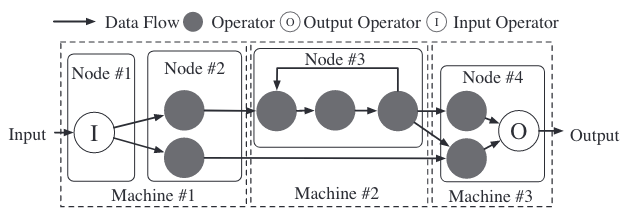
\includegraphics[width=0.95\textwidth]{figures/dataflow.png}
  \end{center}
  \caption{Dataflow Programmierung \cite{baldoniZenohbasedDataflowFramework2021}}
  \label{fig:dataflow}
\end{figure}

In Abbildung \ref{fig:dataflow} ist ein solch Abstraktes Beispiel dargestellt. Knoten 1 hat dabei ein Input Operator der den Datenflow auf zwei weitere Operatoren im Knoten 2 aufteilt. Die Knoten können sich dabei wie dargestellt auf mehreren Maschinen befinden. Knoten vier verbindet den Flow von zwei Operatoren wieder auf in ein Output.\\

Anwendungen können mit diesem Konzept unabhängig der Infrastruktur geplant werden und später mit einem spezielles Framework in die Realität umgesetzt werden. Ein Beispiel für solch ein Framework, ist die von Zenoh sich aktuell in der Entwicklung befindlichen Zenoh Flow Erweiterung. Diese nutzt die bereits behandelten Vorteile von Zenoh und konzentriert sich auf die Umsetzung von den Dataflow Konzepten. Die Umsetzung erfolgt relativ elegant mittels einer Infrastructure as Code Implementierung. Die Knoten und Operatoren werden dabei mit Hilfe einer YAML Syntax in einer deklarativen Art und Weise dargestellt. 

\begin{lstlisting}[caption={Beispiel einer YAML Datei für die Konfiguration von Zenoh Flow \cite{EclipseZenohFlowExamples2022}.}, label={lst:zenohflow}, captionpos=b]
flow: CountingPipeline
operators: []
sources:
  - id : Counter
    uri: file://./target/release/libcounter_source.so
    output:
      id: Counter
      type: usize
sinks:
  - id : PrintSink
    uri: file://./target/release/libgeneric_sink.so
    configuration:
      file: /tmp/generic-sink.txt
    input:
      id: Data
      type: usize

links:
- from:
    node : Counter
    output : Counter
  to:
    node : PrintSink
    input : Data
\end{lstlisting}

In \autoref{lst:zenohflow} wird dabei ein einfacher Zähler mit der Zenoh Flow Syntax beschrieben. Ein \code{Counter} Programm hat dabei einen Output, welcher den aktuellen Wert des Counters entspricht. Dazu gibt es noch ein \code{Sink} Programm welches den Wert als Input annimmt und ausgibt. Die Verbindung beider Objekte wird mittels \code{links} beschrieben.\\
Wie man hier klar erkennen kann, hat der Ansatz mit Hilfe von Infrastructure as Code den Vorteil die Konfiguration wiederverwendbar zu machen. Inspiration gibt es dabei an vielen Cloud Projekten wie Kubernetes oder Terraform die ebenfalls Infrastructure as Code für wiederverwendbare Beschreibungen von Architekturen nutzen.\\

Wie man sich vorstellen kann, eröffnet die Dataflow Programmierung eine noch Einfache Möglichkeit um Systeme wie in im Cloud und Edge Robotics Bereich zu verbinden. Ein Interessanter Use Case wäre die Auslagerung der Auswertung von Sensordaten in die Edge Schicht und die Verwendung der Berechnungsergebnisse wieder im Roboter. Der Roboter und die Edge Instanz wären dabei die beiden Involvierten Knoten. Ein Bewegungssensor im Roboter würde als Informationsquelle dienen, der an ein Output Operator angeschlossen ist. Die Informationen werden dabei zu beliebig vielen Berechnungsoperatoren im Edge geschickt. Nach der Berechnung kommen diese wieder in ein Input Operator am Roboter an und können zur Navigation verwendet werden.\\
Wie man also sehen kann, wendet Zenoh Flow das Konzept der Dataflow Programmierung an um die darunterliegende Infrastruktur soweit wie Möglich zu abstrahieren. Knoten und Operatoren durch \code{sources} und \code{sinks} mit den jeweiligen \code{input} und \code{output} Optionen. Vielversprechend ist auch die Abstraktion der Verbindungen. Diese werden in den \code{links} beschrieben und erstellen ein Zenoh Netzwerk. Die ganzen in dieser Arbeit beschriebenen Details müssen vom Entwickler nicht beachtet werden.

% subsubsection Dataflow Programmierung (end)

% subsection Technologien (end)

\subsection{Fazit} % (fold)
\label{sub:Fazit}

Wie in dieser Arbeit vorgestellt, ist das Thema Cloud und Edge Robotics sehr relevant. Dies lässt sich an verschiedenen Punkten erkennen. Zum einen, gibt es in diesem Bereich ein relativ Schnelllebiges Entwicklungsumfeld. Federführend ist dabei die Eclipse Foundation die hier mehrere Projekte unterstützt. Wie bereits erwähnt, entwickeln sich diese Projekt relativ schnell. Ein gutes Beispiel ist Fog05 ~\cite{EclipseFog052022}. Dieses war als als Ende zu Ende Lösung zum Provisionieren von Netzwerk, Speicher und Rechen Ressourcen in dezentralisierten Infrastrukturen gedacht\cite{corsaroFogO5UnifyingComputing2018}. Fog05 wurde ebenfalls unter der Eclipse Foundation entwickelt und wurde in relativ aktuellen Wissenschaftlichen Veröffentlichungen erwähnt. Trotz dessen, wurde die Entwicklung zu Gunsten des ebenfalls von Eclipse betreuten Zenoh Projektes ruhen gelassen. Projekte rund um Zenoh, wie die bereits erwähnte Zenoh Flow Erweiterung erfreuen sich immer größer werdenden Interesses. Zu sehen, an der aktiven in Entwicklung der Projekte auf dem Code Versionsverwaltungsdienst GitHub. In den dort entwickelten Projekten lässt sich ein positiver Trend in der Entwicklung von Cloud und Edge Robotik Projekten erkennen: Die wichtigsten Entwicklungen in diesem Bereich sind Open Source. Sowohl ROS2 als auch Zenoh und die weiteren in dieser Arbeit vorgestellten Technologien sind frei zur Nutzung verfügbar. Das ist ein wichtiger Faktor um in Zukunft den Bereich schneller wachsen zu lassen.\\

Neben der schnellen Entwicklung im praktischen Bereich, ist auch das Forschungsumfeld sehr aktiv. Im Bereich der Robotik, hat man mit ROS2 eine gute Grundlage gesetzt auf denen weitere Forschungen aufbauen können. Ein Vorteil aus den bereits bestehenden Grundladen, ist die Möglichkeit sich mit Themen zu beschäftigen, die sich mehr auf Nischen konzentrieren. Ein gutes Beispiel ist hier der Forschungsbereich rund um Robotik Systeme. Hier geht es immer mehr in Richtung spezielle Themen wie der Industriellen Anwendung oder dem autonomen Fahren. Dies steht im Gegensatz zu Forschungsergebnisse im Bereich des Edge Computings. Hier basieren viele Paper auf teilweise schon stillgelegte Konzepte wie das bereits erwähnte Fog05.\\

Trotz der positiven Signale im Entwicklungs und Forschungsbereich, ist die Perspektive für die Praxis aktuell noch nicht so klar. Wie in den vorherigen Abschnitten beschrieben, besteht noch kein klares Standard auf das man sich beruhen könnte. Trotz dessen, macht unter anderem die Eclipse Foundation im Edge und Cloud Bereich eine gute Arbeit, in dem es durch Kooperationen, Konferenzen und Projekte versucht Unternehmen auf Standard Technologien zu vereinen. Für die Industrie bedeutet es, dass es aktuell schwer ist sich auf eine bestimmte Technologie festzulegen. Viel mehr, ist es aktuell sinnvoller mit Proof of Concepts aktuelle Technologien zu testen und an der Entwicklung von neuen Möglichkeiten aktiv teilzuhaben.

% subsection Fazit (end)


% -------------------------------------------------------------------------------------------------

% Normaler LNCS Zitierstil
\bibliographystyle{splncs04} % CUSTOM ADDITION OF BIBLIOGRAPHY STYLE
\bibliography{literatur}

\end{document}
